\documentclass[12pt]{article}
\usepackage[utf8]{inputenc}
\usepackage{gensymb}
\usepackage{textcomp}
\usepackage{mathtools}
\usepackage{amssymb}
\usepackage{todonotes}
\usepackage{algorithm}
\usepackage[noend]{algpseudocode}
\newcommand{\mytilde}{\raise.17ex\hbox{$\scriptstyle\mathtt{‌​\sim}$}}
\title{Machine Learning Engineer Nanodegree Capstone Project}
\author{Mateusz Bednarski}
\date{\today}


\usepackage{graphicx}
\graphicspath{ {images/} }

\DeclareMathOperator*{\argmax}{arg\,max}
\usepackage{hyperref}


\begin{document}

\maketitle



\section{Introduction}

Domain for my capstone project is control problems or robot motion. This requires either a physical robot or simulation engine. For purposes of this project I decided to make use of OpenAI Gym\cite{GYM}. Gym is set of environments simulating various tasks. It provides ready to use simulators and frameworks for comparing algorithms. From available environments, I have selected "LunarLander-v2"\cite{lunarlander}. For a few reasons:
\begin{itemize}
\item For first, reinforcement learning interested me the most, so I want to get deeper into this.
\item OpenAI provides leaderborads for each environement, making result comparison easy.
\item OpenAI provides problem implementations, thus I can focus only on RL part.
\item I love space and landing on a planet/moon is interesting problem for me.
\item It has (approximately – more details in dataset section) continuous state space, so basic tabular Q-learning will not work – I need to examine more sophisticated techniques.
\item Lunar lander is quite challenging environment.
\end{itemize}

\section{Problem Statement}

\begin{figure}[h]
\centering
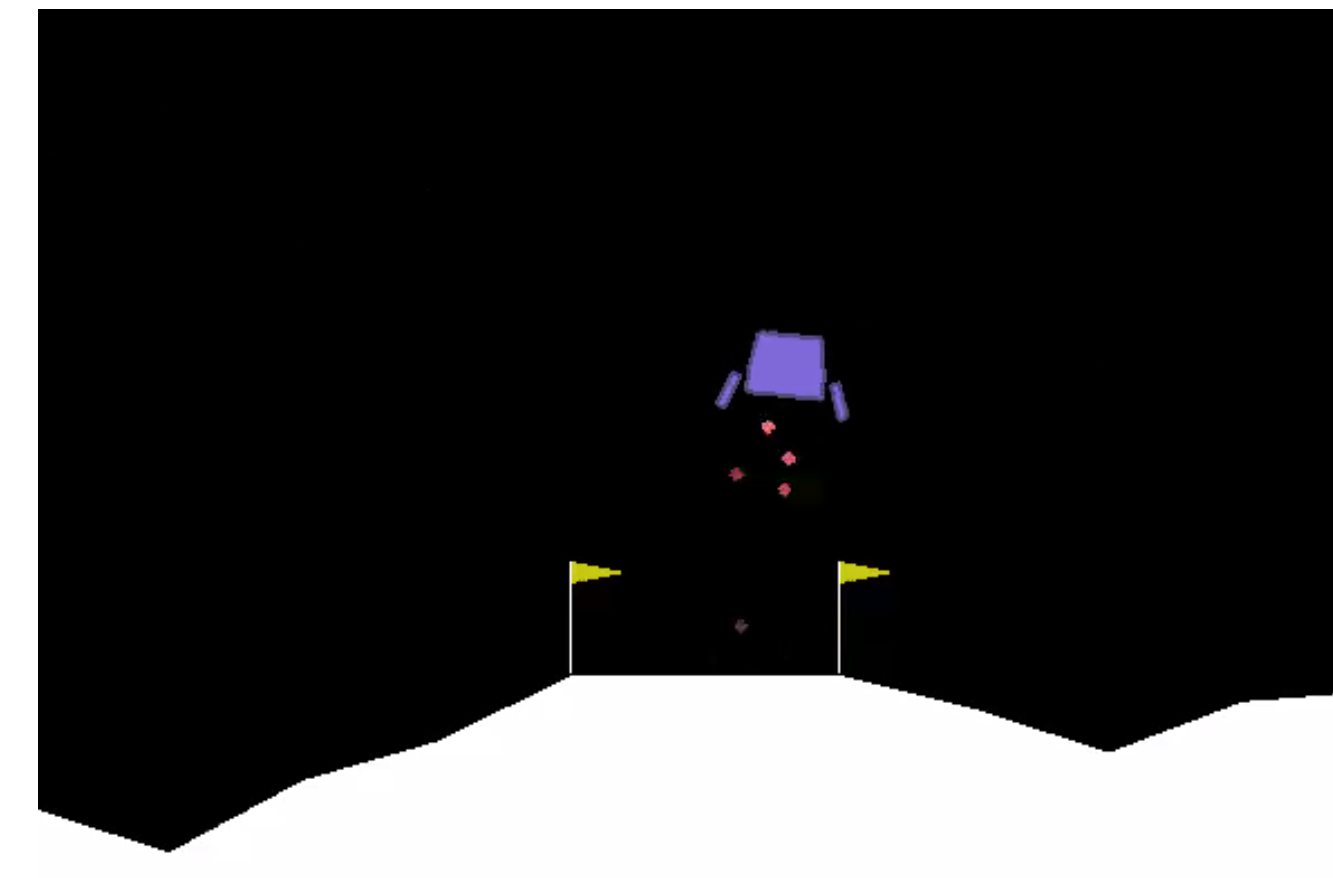
\includegraphics[scale=0.3]{lunar.png} 
\caption{Screenshot from the environment}
\end{figure}


There are a landing pad and a lander. Lander has two legs, and three engines – thrust directed down, left and right. Possible actions are one of do nothing/fire main engine/fire left engine/fire right engine.  Task is to land on the landing pad.  Lander starts above the pad and is affected by gravity. Simulation is finished either lander lands or crashes. Landing outside pad is also possible. Fuel is unlimited and there is no time penalty.
Rewards and penalties are already defined in the environment:
\begin{itemize}
\item Moving towards pad with zero speed: from $+100$ to $+140$
\item Crash: $-100$
\item Successful landing: $+100$
\item Leg with ground contact: $+10$
\item Firing main engine (not side engine): $-0.3$
\item When landing outside pad, an additional penalty is given.
\end{itemize}

Environment is considered as solved, when average episode reward for 100 consecutive episodes is at least 200.

\subsection{Evaluation metric}

For measuring performance I will use number of episodes until solving the environment and time to reach it. This is because I suppose, that some approaches may perform more, faster episodes when others conversely - less, longer episodes.

\section{Analysis}
\subsection{Data Exploration}

As it is a reinforcement learning problem, there is no dataset understood in classical way.

\subsubsection{Action and state space}

Action space is a discrete, finite set:

\begin{equation}
\begin{aligned}
&A = {0,1,2,3} \\
&|A| = 4
\end{aligned}
\end{equation}

State space is a vector of 8 real numbers describing lander position, velocity and orientation. Last two components says if left and right lander leg touch ground. If so, they are set to 1, instead - 0.

\begin{equation}
\begin{aligned}
&S \in \mathbb{R}^8 \\
&s_{0..5} \in (-\infty, +\infty) \\
&s_{6,7} \in \{0,1\} \\
\end{aligned}
\end{equation}

\subsubsection{Space size}

Before, I said that space consists of real numbers. Given that, space state size  would be uncountably infinite. However, during to machine representation of real numbers it is not exactly true. In typical implementation, \emph{float} can handle one of $2^{52}$ values \footnote{\url{http://stackoverflow.com/a/8875223}}. Size of Q-table for LunarLander is:

\begin{equation}
|Q| = |S \times A| = |S| \times |A| = \underbrace{{(2^{52})}^6 \cdot 2^2}_{|S|} \cdot \underbrace{4}_{|A|} \approx 2.24 \cdot 10^{102}
\end{equation}

Which requires $9 \cdot 10^{89}$ PB of memory. Also, each state should be visited enough number of times. It definetely makes this unsolvable by tabular Q-learning.

\subsection{Algorithms}

Because Q-space ($S \times A$) is infinite in size, it is impossible to use Q lookup table. There are many approaches to deal with this problem. Basic two approaches to deal with this problem is approximation and discretization. Approximation is to replace Q table with a function $h(s,a) \rightarrow \mathbb{R}$, that will approximate $Q(s, a)$ values. Therefore, the goal is to find a function $h(s, a)$, that will return a Q-value for a given pair $(s,a)$. 
Discretization combines ranges of continuous space state into discrete buckets. However, I decided to use completely different approach.

\subsection{Parameter-exploring Policy Gradient}
Instead of using techniques that are focused on searching function approximating q-values, Parameter-exploring Policy Gradients\cite{pgpe} uses \emph{policy space}. As Ultimate goal is to find a policy that will solve the environment this algorithm search the policy space in order to find such one.

PEPG is a policy gradient method, it does mean that it estimates policy gradient and use it to maximize rewards given by following a policy.

For purposes of this project I have implemented this algorithm with slight differences.

\subsubsection{Policy}

For first, we define a parametrized policy $\pi_\theta$

\begin{equation}
\pi_\theta: s \rightarrow a
\end{equation}

For this PGPE, the policy can be basically free-form. I used two layered feed-forward neural network. (one hidden layer, and one output layer).
Hidden layers contains 32 neurons. Output layer has 4 neurons - one per possible action. All layers has $\tanh$ activation function.

If we denote $x$ as state, $\theta = (W,b,W_2,b_2)$ as policy parameters, the whole policy is following:

\begin{equation}
\begin{aligned}
z &= xW + b \\
\varphi &= \tanh(z) \\
z_2 &= \varphi W_2 + b_2 \\
\varphi_2 &= \tanh(z_2) \\
\text{selected action} &= \argmax(\varphi_2)
\end{aligned}
\end{equation}

There is no need to backpropagate this network.

\subsubsection{Definitions}

\begin{itemize}

\item $\theta$ is policy parametrization (one-dimensional vector)

\item $P$ in size of parametrization $\theta$. $\theta \in \mathbb{R}^P$

\item $\mathcal{N}(\mu, \sigma^2)$ is normal distribution with mean $\mu$ and variance $\sigma^2$

\item $\mu$ is current mean parametrization

\item $T$ and $S$ are matrices with shape $P\times N$

\end{itemize}

\subsubsection{Parameters}

\begin{itemize}
\item $N$ is a size of the population
\item $\alpha_\mu, \alpha_\sigma$ are learning rates
\item $H$ is history size
\item $\sigma$ is initial standard deviation for policy parameters

\end{itemize}

\subsubsection{Algorithm}

\begin{algorithm}
\caption{PGPE for LunarLander-v2}
\begin{algorithmic}[1]
\State initialize $\mu$ with zeros
\State test phase $\gets$ false
\While{not solved}
	\If{test phase}
		\State validation score $\gets$ evaluate policy($\mu$)
		\State continue
	\EndIf
	\For {$n=0$ to $N-1$}
		\State sample $\theta^{(n)}$ from $\mathcal{N}(\mu, \sigma^2)$
	\State $R^{(n)} \gets$ evaluate policy($\theta^{(n)}$)
	\EndFor
	\State $T_{ij} \gets \theta_i^{j} - \mu_i$
	\State $S_{ij} \gets \frac{T_{ij}^2 - \sigma_i^2}{\sigma_i}$
	\State $R^{(n)} \gets R^{(n)} - b$
	\State validation score $\gets$ evaluate policy($\mu$)
	\State b $\gets$ mean reward of last $H$ iterations
	\If{mean validation score for last 20 is greater than 200}
		\State{test phase $\gets$ true}
	\EndIf
	\State $\mu \gets \alpha_\mu \mu TR$
	\State $\sigma \gets \alpha_\sigma \sigma SR$
\EndWhile

\end{algorithmic}
\end{algorithm}

Algorithm works in two phases. During first (training phase) in every iteration it evaluates population of $N$ policies and updates $\mu$ and $\sigma$. For each iteration, policy parametrized by $\mu$ is evaluated separately. It does not affect learning, instead measures current performance. If for 20 consecutive trials, validation reward is greater than 200 (it is threshold for solving) we assume that parametrization $\mu$ is sufficient and we can go to test phase.

In test phase, we use learned parametrization $\mu$ in order to get 100 solved episodes. This is done for optimalization - as correct policy was found there is no need to evaluate $N$ policies every time anymore.


\subsection{Benchmark}

For benchmark I have selected following evaluation from gym - \url{https://gym.openai.com/evaluations/eval_QOfhB9uhQ1W2hKqF8H365A} by user @pranz24. This algorithm (Covariance Matrix Adaptation Evolution Strategies) solved environment after 60199 episodes and 3 hours. I will use it to compare with outcome of my work.

\section{Methodology}
\subsection{Data Preprocessing}

No form of preprocessing was done in this project as it was not required. However, in general RL can use data preprocessing in order to represent observations in more suitable way (e.g.: tile coding, RBF coding, continuous values discretization).

\subsection{Implementation}

\subsubsection{Parallelization}

Some part of the algorithm can be easily parallelized - loop at lines 7-9. This is because each iteration in population is independent from another. Created implementation utilizes this possibility. For parallelizsm, library \texttt{joblib} was used. As a result, execution time is reduced 2-3 times.

Algorithm was implemented in two classes - \texttt{NeuralNetPolicy} and \texttt{PGPEAgent}

\texttt{NeuralNetPolicy} responsibility is to select an action basing on given state and policy parametrization. Interface is following:

\begin{itemize}
\item  Constructor takes number of features, actions and sizes for hidden layers

\item \texttt{unpack} gets 1D vector and extract weights for neurons 

\item \texttt{get\_number\_of\_parameters} computes total number of parameters (this is size for $\theta$)

\item \texttt{forward\_pass} performs forward pass for given parametrization and state. Returns action to perform.
\end{itemize}

\texttt{PGPEAgent} implements the algorithm. Constructor takes all required parameters (environemnt to solve, $\alpha_\sigma$, $\alpha_\mu$, $\sigma$, size of history and population, number of test iterations. It contains two methods.

\begin{itemize}

\item \texttt{run} takes maximum number of episodes to perform. it implements PGPE and basic visualization plotted in real time.

\begin{figure}[h]
\centering
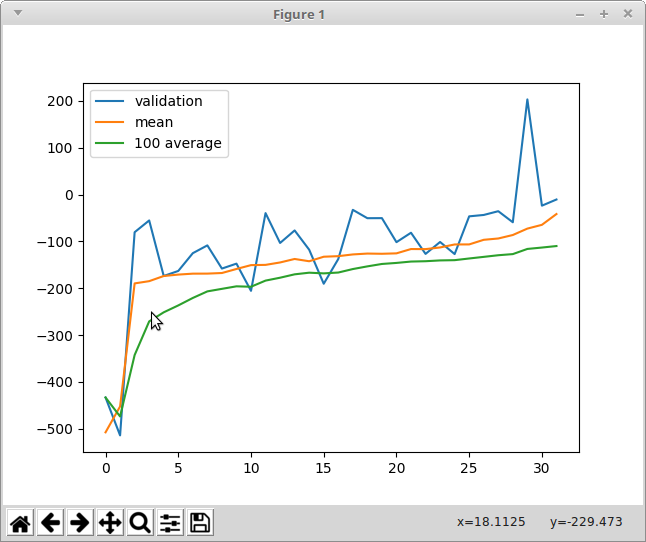
\includegraphics[scale=0.5]{monitor.png} 
\caption{Visualization during training}
\end{figure}

\end{itemize}

\texttt{evaluate\_policy} performs full episode using given parametrization $\theta$. This function is not member of any class because of it will be runned in parallel - \texttt{joblib} requires such code  not to be a class method.

Apart of them \texttt{Monitor} class was implemented. This class is responsible for saving duration and reward for episodes and store them into files. Next, they can be used to generate statistics and plots (\texttt{analysis.py}).

\subsection{Complications and Refinement}

Solution improvements came along with solving issues, so I am presenting them in a single list.

\begin{itemize}
\item{\textbf{Policy}} Initially, two layer neural network policy was used (both layers with size of 32 neurons). This approach caused slower divergence in aspect of iterations to solve (more parameters was needed to tune) and iteration duration (more computations for forward pass). Later one it turned out, that simpler policy is also capable for this problem and reduces training effort. However, with removing hidden layer completely I was not able to get solution. Learning: policy should be just as complicated as required, making it more sophisticated does not provide any benefit.

\item{\textbf{GPU utilization}} To make process even faster I have tried to perform some computations on GPU. For this I have implemented policy forward pass using TensorFlow\cite{tensorflow} using various scenarios (creating computation graph at once and use \texttt{tf.placeholder} to set weights, creating graphs multiple times with \texttt{tf.constant}). However, it resulted with worse execution times. I did not perform specific profiling, but I believe there were too little computations to equilibrium cost of CPU/GPU communication.

\item{\textbf{Another Python distribution}} Another attempt to optimize the code, was to use Intel Python Distribution\footnote{https://software.intel.com/en-us/intel-distribution-for-python} but results were unnoticeable.

\item{\textbf{Floating point errors}} Initially I have used much higher learning rates. Learning was faster, but I have experiencing floating point arithmetic errors - policy parameters quickly became too high causing overflow errors. This forced me to use \texttt{np.seterr('raise')} in order to be notified about those errors.

\item{\textbf{Random number generator}} A lot of issues occurred when I tried to generate random numbers in threads. Given that, final implementation computes random numbers in main thread and send them to worker threads.

\end{itemize}



\section{Model evaluation}

\subsection{Measured qualities}

For each test, two qualities was measured: number of iterations and total execution time (computed as sum of all iteration times). They are the same as in Evaluation metric section.

\subsection{Parameters}

Parameters are also same as shown before. Quick recap:

\begin{itemize}
\item $N$ is population size
\item $\alpha_\mu, \alpha_\sigma$ are learning rates
\item $H$ is history size
\item $\sigma$ is initial standard deviation for policy parameters

\end{itemize}

Most comprehensive way to perform analysis would be to run grid search over whole parameter space with few repetitions - in order to reduce fluctuations influence. However, with regard to long execution time it was impossible. Instead, I established a baseline set of parameters and measured influence of each parameter separately. The baseline parameters are following:

\begin{table}[!h]
\centering
\begin{tabular}{|c|c|}
\hline 
Parameter & baseline value \\
\hline 
$N$ & $500$ \\
\hline 
$\alpha_\mu$ & $1 \cdot 10^{-4}$ \\
\hline 
$\alpha_\sigma$ & $1 \cdot 10^{-5}$ \\
\hline 
$H$ & $50$ \\
\hline 
$\sigma$ & $0.5$ \\
\hline 
\end{tabular} 
\caption{Baseline parameters}
\end{table}

As there are 5 parameters, 10 configurations were created - with bigger and smaller value of each one. Parameters values for those settings are described in Table 2.

\begin{table}[!!h]
\centering
\begin{tabular}{|c|c|c|c|c|c|c|c|c|}
\hline 
\# & $N$	& $\alpha_\mu$	& $\alpha_\sigma$	& $H$	& $\sigma$ &	time to finish [min]&	iterations to finish & it/min\\
\hline
0 & 500     &  0.0001	& 0.00001	& 50	& 0.5	& 23.15 &	55   & 2.3 \\
1  & 400	&  0.0001	& 0.00001	& 50	& 0.5	& 15.78 &	91   & 5.7\\
2  & 600	&  0.0001	& 0.00001	& 50	& 0.5	& 25.29 &	49   & 1.9\\
3  & 500	&  0.0002	& 0.00001	& 50	& 0.5	& 30.96 &	113  &  3.65\\
4  & 500	&  0.00005	& 0.00001	& 50	& 0.5	& 25.86 &	253  &  9.78\\
5  & 500	&  0.0001	& 0.00002	& 50	& 0.5	& 23.22 &	47   & 2.02\\
6  & 500	&  0.0001	& 0.000005 & 	50 	& 0.5	& 27.78 &	78   & 2.80\\
7  & 500	&  0.0001	& 0.00001	& 75	& 0.5	& 29.14 &	88   & 3.02\\
8  & 500	&  0.0001	& 0.00001	& 25	& 0.5	& 29.54 &	75   & 2.53\\
9  & 500	&  0.0001	& 0.00001	& 50	& 0.6	& 24.87 &	91   & 3.66\\
10 &  500&     0.0001	& 0.00001	& 50	& 0.4	&  27.5 &	52   & 1.89\\
\hline
\end{tabular} 
\caption{Parameters exploration}
\end{table}
Fist of all results show that indeed higher number of iterations does not imply longer execution time - e.g. comparing \#0 with \#1. After this, selected baseline looks like being near to the optimum (at least local one ).

Reducing size of population (\#0,1,2) causes almost twice as much iterations to perform, but they are a lot of faster. This is because in later stage of learning when models performs better also execution time increases - lander stops crashing fast. As expected increasing $N$ makes fewer, longer iterations.

Both learning rates (\#0,3,4,5,6) seems to be near optimum, because changing them makes process longer. Especially reducing $\alpha_\mu$.

Similar effect can be observed for $H$ (\#7,8).

Increasing initial $\sigma$(\#9,10) causes big incrementation in terms of iterations and reducing - in time. 


In project repository, there are plots for all of those configurations (parameter exploration directory).


In order to provide more complete and reliable analysis for each case multiple runs should be executed. Also, relations between parameters may be explored. This could be done either by hand or using GridSearch or RandomSearch from scikit-learn\cite{sklearn} over parameter space. However it was done because of lack of available computation time.

In fact, for all parameters model was able to solve the task.

\subsection{Results and visualization}

In results analysis I will use baseline parameter values. Implemented model finished learning phase after 55 iterations and approximately 23 minutes. As population size was set to 500, this gives actual number of simulation episodes  $55 * 500 = 27500$. After learning phase there were 200 test runs (without learning). To sum up, agent achieved "average for 100 consecutive trials above 200" at iteration \textbf{21} after total number of episodes equal to $21 * 500 = 10500$. So here is the point when environment can be considered as solved (even if agent was learning longer).

\begin{figure}[!h]
\centering
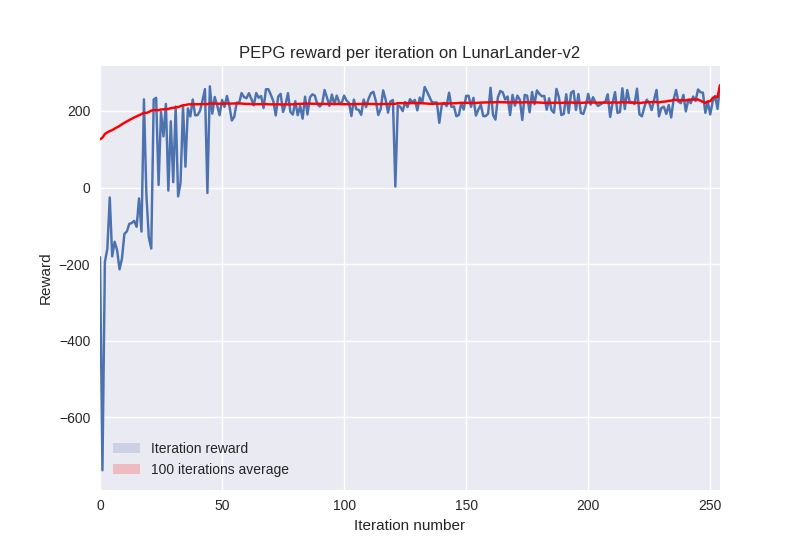
\includegraphics[scale=0.9]{final_plot.png} 
\caption{Agent rewards per iteration}
\end{figure}

\begin{figure}[!h]
\centering
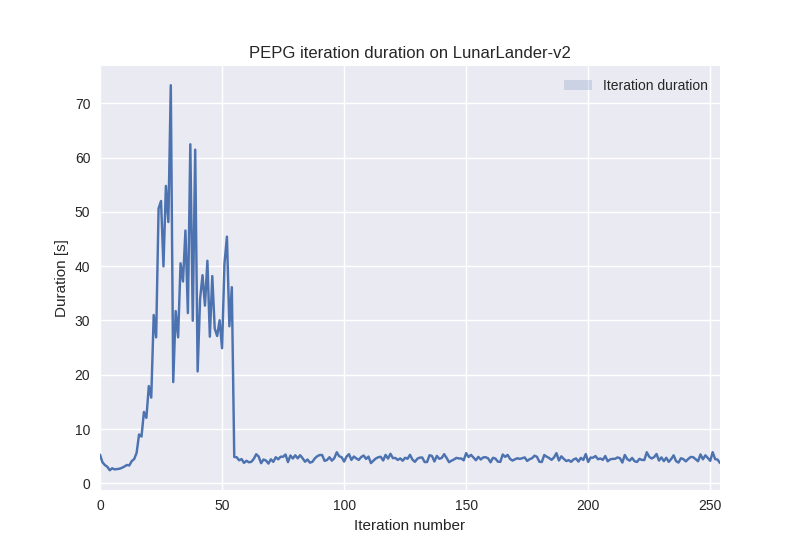
\includegraphics[scale=0.9]{final_plot_duration.png} 
\caption{Iteration durations}
\end{figure}

When it comes to iteration duration time it can be seen that during learning phase this time is a lot of longer due to fact that on testing phase there is only one episode instead of few hundreds.

Repeating model executions give similar results.

\subsection{Justification}

Presented model performed better than one selected in benchmark section. To recap benchmark model solved problem after 60199 episodes in about 3 hours, when presented here required only 10500 and 23 minutes.

\subsection{Hardware}
Hardware environment used in this project is Intel i5 3,1GHz CPU with 16GB RAM memory and Linux Mint 18.1 x64.

\section{Conclusion}
\subsection{Reflection}

To put it briefly: I have implemented the PEGP algorithm in multi-threaded version in order to solve LunarLander-v2 reinforcement learning problem. Implemented solution uses feed forward neural network with one hidden layer and does not require backpropagation. I am satisfied with achieved results. I found aspect of optimizing code very interesting even if I was not able to utilize GPU. Another interesting thing was to actually research algorithms that could help me - at some point I wanted to give up because I had feeling, that I will not be able to complete this project.

\subsection{Improvement}

PEPG algorithm can benefit from technique called \emph{symmetrical sampling}. Briefly it generates random perturbations ($\epsilon$) on current policy($\mu$ and apply as addition and a subtraction, resulting in two populations - $\mu - \epsilon$ and $\mu + epsilon$). This makes gradient estimation more precise and reduces variance. However this makes implementation more complicated and due the fact that I am satisfied with current results I did not decide to implement this.

Another improvement could be deeper parameter exploration (as mentioned earlier).


\newpage

\bibliographystyle{alphaurl}
\bibliography{references} 

\end{document}

